\section{Theorie}
\label{sec:Theorie}
Im Folgenden werden die Grundzüge der Theorie der thermischen Eigenschaften von Festkörpern erläutert. Die Erklärungen basieren hauptsächlich auf den Ausführungen in Kapitel 6 aus dem Buch "Festkörperphysik" von Rudolf Gross und Achim Marx \cite{grossMarx}.

\subsection{Definition der Wärmekapazität}
\label{sec:definitionWaermekapazität}
Für die Wärmekapazität eines Festkörpers gilt
\begin{equation}
  C = \frac{\Delta Q}{\Delta T}\,,
  \label{eqn:C}
\end{equation}
wobei $\Delta Q$ die Wärmemänge ist, die nötig ist, um die Temperatur des Körpers um $\Delta T$ zu erhöhen.\\
Die Größe $C$ ist extensiv. Um eine intensive, nur vom Stoff abhängige Größe zu erhalten, kann sie durch eine andere extensive Größe geteilt werden, um eine sogenannte spezifische Wärmekapazität zu erhalten. Ein Beispiel dafür wäre die molare spezifische Wärmekapazität $c^{\text{mol}} = \frac{C}{n}$ mit der Stoffmenge $n$.

Der erste Hauptsatz der Thermodynamik formuliert eine verallgemeinerte Energieerhaltung als
\begin{equation}
  \text{d}U = \delta Q + \delta W = \delta Q - p \text{d}V\,.
  \label{eqn:ersterHauptsatz}
\end{equation}
Dabei ist $U$ die innere Energie, $Q$ die Wärmemenge und $W$ die Arbeit. Differenzielle Änderungen dieser Größen sind mit $\text{d}$ und $\delta$ gekennzeichnet.\\
Im Allgemeinen hat die Änderung der Temperatur $T$ des Körpers auch Folgen für andere Zustandsvariablen wie den Druck $p$ oder das Volumen $V$. Es ist allerdings oft möglich, diese Variablen durch externe Einflüsse konstant zu halten. Befindet sich der Körper während der Wärmezufuhr zum Beispiel an der Luft, so findet diese bei konstantem Druck, dem Luftdruck, statt. Es könnte auch das Volumen konstant gehalten werden, indem der Körper eingeschlossen wird, sodass keine thermische Ausdehnung stattfinden kann.\\
Es ergeben sich für diese beiden Fälle verschiedene Wärmekapazitäten, die durch ein Subskript gekennzeichnet und allgemeiner mithilfe von Ableitungen definiert werden. Der Grund für den Unterschied ist folgender: Bei Wärmezufuhr bei konstantem Druck wird ein Teild er zugeführten Wärme in Arbeit für die thermische Ausdehnung umgewandelt. Dies ist bei Wärmezufuhr bei konstantem Volumen nicht der Fall, weswegen $C_p$ bei reellen, nicht idealisierten Körpern stets größer als $C_V$ ist. Dieser Effekt ist bei Gasen größer als bei Festkörpern, da Gase eine größere thermische Ausdehnung als Festkörper ausweisen.
Unter Betrachtung von Gleichung \ref{eqn:ersterHauptsatz} lassen sich die Wärmekapazitäten durch
\begin{align}
  C_V &\equiv \left(\frac{\delta Q}{\partial T}\right)_V = \left(\frac{\partial U}{\partial T}\right)_V\, \label{eqn:C_V}\\
  C_p &\equiv \left(\frac{\delta Q}{\partial T}\right)_V \label{eqn:C_p}
\end{align}
definieren.\\
Für den Zusammenhang zwischen den beiden Wärmekapazitäten gilt
\begin{equation}
  C_p - C_V = V T \frac{\alpha^2}{\kappa_T}\,.
  \label{eqn:CpminusCV}
\end{equation}
Dabei sind $\alpha \equiv \frac{1}{V}\left(\frac{\partial V}{\partial T}\right)$ der thermische Expansionskoeffizient und $\kappa_T \equiv - \frac{1}{V}\left(\frac{\partial V}{\partial p}\right)$ die isotherme Kompressibilität. Es ist möglich, diese Formel geeignet zu modifizieren, um spezifische Wärmekapazitäten zu betrachten.\\
In der experimentellen Praxis ist es deutlich leichter, bei konstantem Druck als bei konstantem Volumen zu messen, da enorme Kräfte nötig wären, um die thermische Expansion des Materials über große Temperaturbereiche zu verhindern. Deswegen ist die obige Formel für die Auswertung von Experimenten für Bedeutung, da sie die Verbindung zwischen der experimentell berechnbaren Größe $C_p$ und der theoretisch vorhergesagten Größe $C_V$ darstellt.

\subsection{Modelle zur Berechnung der Wärmekapazität}
\label{subsec:modelleWaermekapazitaet}
\subsubsection{Klassische Betrachtung}
Es sollen im Folgenden nur Festkörper betrachtet werden. Diese bestehen aus Atomen, die über Ruhelagen auf ihren Gitterplätzen verfügen und rückwirkenden Kräften ausgesetzt sind, falls sie aus der Gleichgewichtslage ausgelenkt werden. Es liegt eine translatorische Symmetrie vor, sodass sich eine Elementarzelle mit $r'$ Atomen definieren lässt, welche periodisch fortgesetzt den vollständigen Festköper ergibt. Folglich lässt sich der Festköper durch $r'N$ gekoppelte harmonische Oszillatoren mit Schwingungsmöglichkeiten in allen drei Raumdimensionen beschrieben werden.\\
In der klassischen Physik gilt der Gleichverteilungssatz: Der Mittelwert jedes in Ort oder Impuls quadratischen Terms in der Hamiltonfunktion beträgt $k_\text{B} T / 2$. Für die Hamiltonfunktion des harmonischen Oszillators gilt
\begin{equation}
  H = \frac{\vec{p}^2}{2 m} + \frac{1}{2} m \omega^2 \vec{r}^2\,,
  \label{eqn:hamilton}
\end{equation}
wobei $\vec{p}$ der klassische Impulsvektor ist,
$m$ bezeichnet die Masse des Atoms, $\omega$ die Kreisfrequenz der harmonischen Schwingung und $\vec{r}$
den Ortsvektor des Teilchens im dreidimensionalen Raum ist. Es liegen also drei quadratische Orts- und drei quadratische Impulsterme pro Atom im Festkörper vor, sodass sich die innere Energie als Mittelwert der Hamiltonfunktion zu $U = 3 r' N k_\text{B} T$. Mit der Definition \eqref{eqn:C_V} ergibt sich die klassiche Vorhersage für die Wärmekapazität eines Festkörpers. Sie wird auch Dulong-Petit-Gesetz genannt. In der molaren spezifischen Wärmekapazität formuliert lautet es
\begin{equation}
  c^{\text{mol}} = 3 R\,.
  \label{eqn:dulongpetit}
\end{equation}
Insbesondere ist die Wärmekapazität in dieser klassichen Betrachtung grundsätzlich temperaturunabhängig. Bei Raumtemperatur ist dies für viele Materialien eine gute Näherung.

\subsubsection{Das Einstein-Modell}
Das Dulong-Petit-Gesetz versagt bei tiefen Temperaturen deutlich. Dort muss die Wärmekapazität wegen einer Folgerung aus dem dritten Hauptsatz der Thermodynamik gegen null gehen, was in experimentellen Beobachtungen auch bestätigt wird.\\
Zur Wärmekapazität eines Festkörpers tragen sowohl Elektronen bei, welche sich quasifrei durch ein schwaches periodisches Gitterpotenzial als eine Art Gas im Festkörper aufhalten, als auch die Gitterschwingungen, die quantenmechanisch als Quasiteilchen, sogenannte Phononen, interpretiert werden. Der elektronische Anteil kann zwar nicht vernachlässigt werden, jedoch spielt er nur für tiefe Temperaturen, wo viele Moden der Gitterschwingungen nicht angeregt ("eingefroren") sind, eine signifikante Rolle und wird im Folgenden nicht weiter betrachtet.

Die Phononen verfügen über Dispersionsrelationen und es gibt im Allgemeinen zwei Arten von Phononen, die Optischen und die Akustischen. Es gibt drei akustische Zweige und $3r-3$ optische Zweige, wenn $r$ die Anzahl an Atomen in der Elementarzelle ist. Die Dispersionsrelationen sind in Abbildung \ref{fig:phononen} skizziert.

\begin{figure}
  \centering
  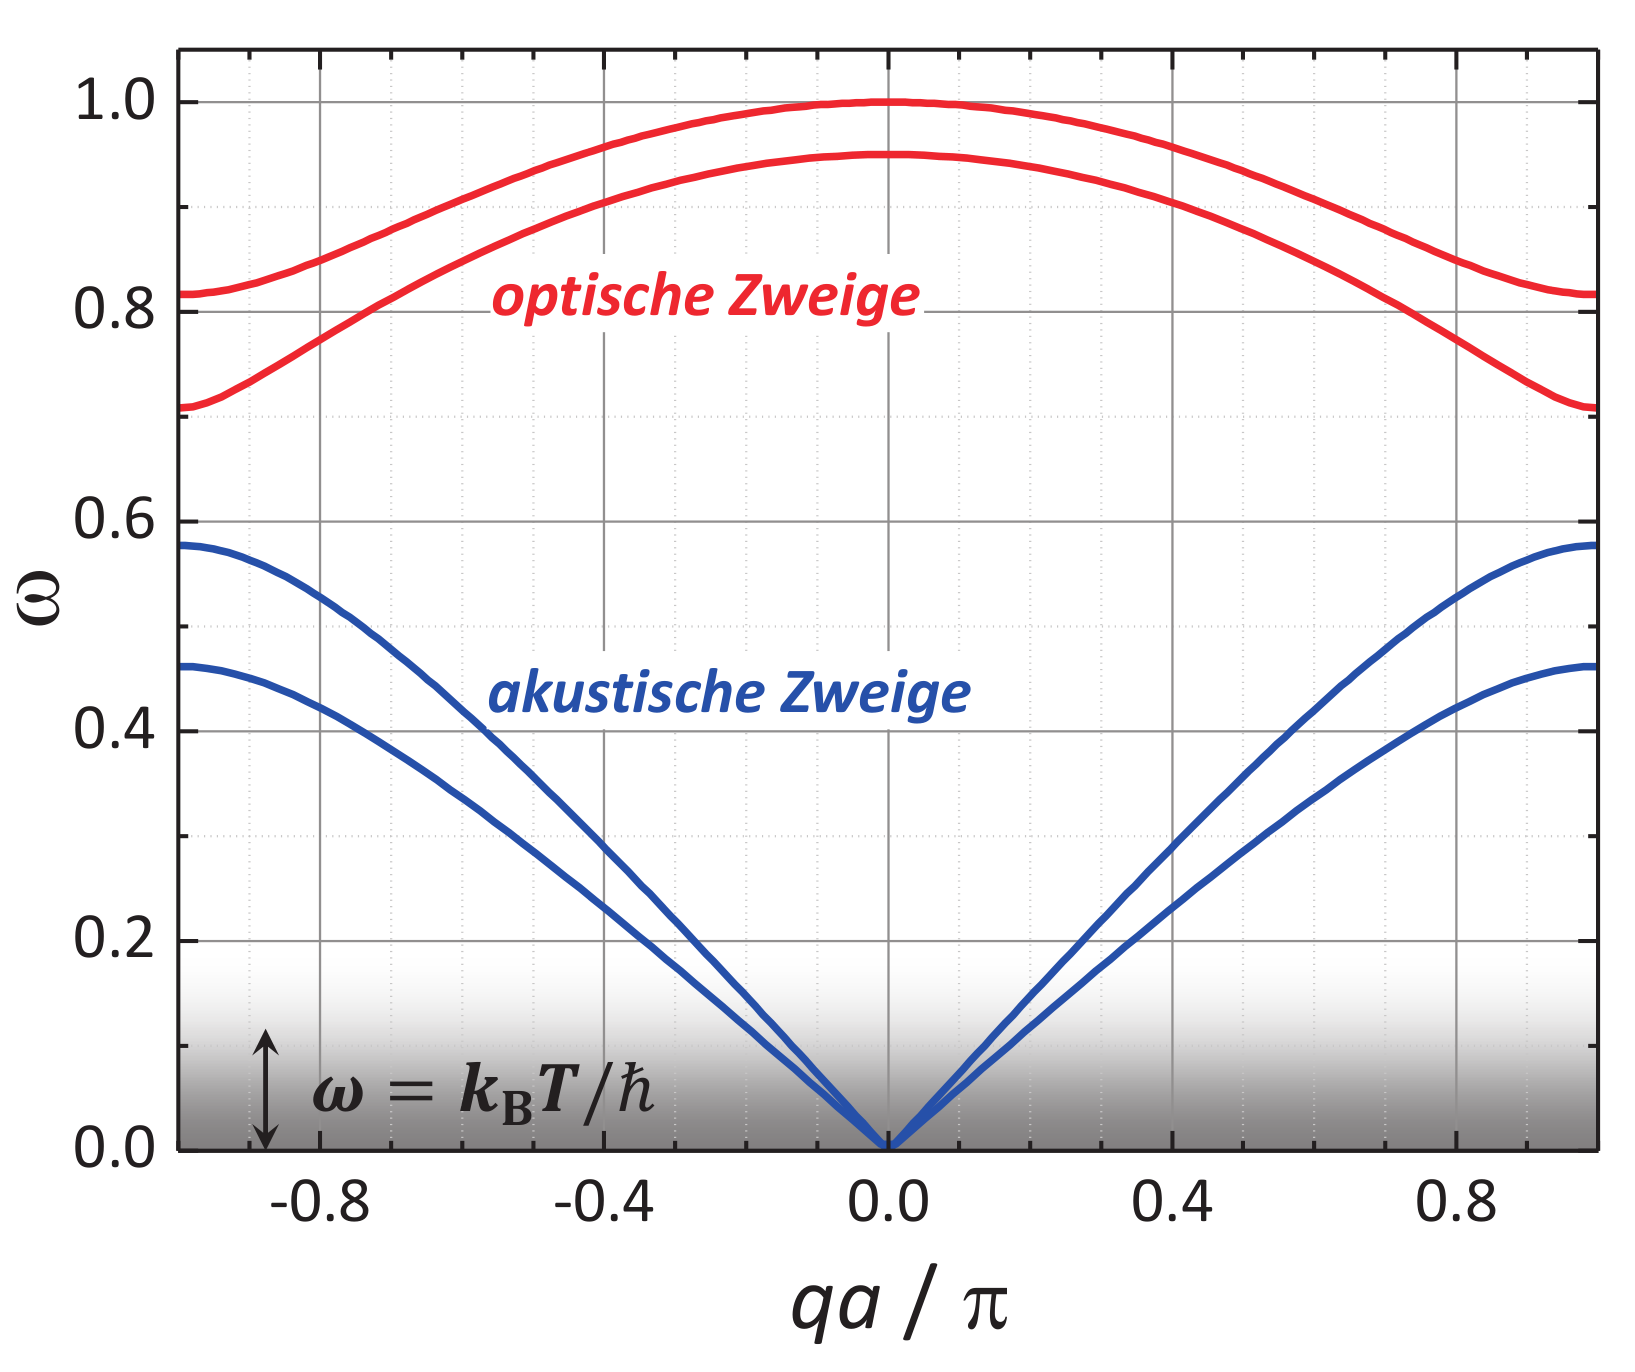
\includegraphics[width=300pt]{data/phononen.png}
  \caption{Darstellung der verschiedenen Dispersionsrelationen der Phononen in Abhängigkeit ihres Wellenvektors \cite{grossMarx}.}
  \label{fig:phononen}
\end{figure}

Im Einstein-Modell wird angenommen, dass die Gitteratome mit nur einer Kreisfrequenz $\omega_\text{E}$ schwingen. Im Folgenden wird der Einfachheit eine einatomige Basis angenommen.

Im Allgemeinen hängt die Besetzung der Phononenzustände von der Temperatur ab. Da Phononen Bosonen sind, gilt für die Besetzungswahrscheinlichkeit die Bose-Einstein-Verteilung
\begin{equation}
  \langle n \rangle = \frac{1}{\exp\left(\frac{\hbar \omega_\text{E}}{k_\text{B} T}\right)-1}\,.
  \label{eqn:boseEinstein}
\end{equation}
Für die innere Energie $U$ im Festkörper gilt dann gemäß der Lösung des harmonischen Oszillators der Quantenmechanik
\begin{equation}
  U = \hbar \omega_\text{E} \langle n \rangle = \frac{1}{\exp\left(\frac{\hbar \omega_\text{E}}{k_\text{B} T}\right)-1}\,.
  \label{eqn:uEinstein}
\end{equation}
Zur Vereinfachung folgender Ausdrücke wird die Einstein-Temperatur als $\Theta_\text{E} = \hbar \omega_\text{E}/k_\text{B}$ definiert.
Die Wärmekapazität bei konstantem Volumen lässt sich durch Ableiten berechnen:
\begin{equation}
  C_V^{\text{E}} = 3 N k_\text{B} \left(\frac{\Theta_\text{E}}{T}\right)^2 \frac{\exp(\Theta_\text{E}/T)}{(\exp(\Theta_\text{E}/T)-1)^2}\,.
  \label{eqn:cVEinstein}
\end{equation}
Durch Entwickeln der Exponentialfunktion ist ersichtlich, dass sich für große Temperaturen $T \gg \Theta_\text{E}$ das Dulong-Petit-Gesetz ergibt, was eine experimentelle Bestätigung des Einstein-Modells für diesen Temperaturbereich bedeutet. Für tiefe Temperaturen $T \ll \Theta_\text{E}$ sagt das Einstein-Modell einen exponentiell abfallenden Verlauf der Wärmekapazität vorher. Der starke Abfall gegen 0 für $T$ gegen 0 ist zwar qualitativ korrekt, im Experiment ergibt sich jedoch für viele Materialien ein weicheres $T^3$-Verhalten. Das quantative Versagen des Einstein-Modells im Tieftemperaturlimes ist dadurch begründet, dass in diesem Bereich die akustischen gegenüber den optischen Phononen, die eine nahezu konstante Dispersionsrelation aufweisen, dominieren.

\subsubsection{Das Debye-Modell}
Das Debye-Modell versucht die Schwächen des Einstein-Modells zu beheben, indem eine lineare Dispersionsrelation mit isotroper Frequenz angesetzt wird. Dadurch wird sich ein besseres Verhalten im Tieftemperaturbereich versprochen, da die akustischen Phononen besser angenähert werden.
Unter diesen Annahmen ergibt sich die innere Energie schließlich zu
\begin{equation}
  U = 9 N k_\text{B} \frac{T^4}{\Theta_\text{D}^3}\int_0^{\Theta_\text{D}/T} \symup{d}\,x \frac{x^3}{\exp(x)-1}\,.
  \label{eqn:uDebye}
\end{equation}
Dabei ist $\Theta_\text{D}$ die Debye-Temperatur. Sie kann ungefähr als Phononenenergie der Mode mit minimaler Wellenlänge interpretiert werden. Damit ist die Debye-Temperatur gerade die Temperatur, bei der alle Moden angeregt sind.\\
Die Wärmekapazität folgt durch Ableitung der inneren Energie nach der Temperatur:
\begin{equation}
  C_V = 9 N k_\text{B} \frac{T^3}{\Theta_\text{D}^3}\int_0^{\Theta_\text{D}/T} \symup{d}\,x \frac{x^4}{(\exp(x)-1)^2}\,.
  \label{eqn:cVDebye}
\end{equation}
Diese Funktion wird auch Debye-Kurve $f\left(\frac{T}{\Theta_\text{D}}\right)$ genannt.
Das Integral ist nichtelementar, weswegen die konkrete Auswertung dieser Funktion in der Regel numerisch geschieht. \\
Für tiefe Temperaturen $T \ll \Theta_\text{E}$ ist das Integral ungefähr
\begin{equation}
  \int_0^{\infty} \symup{d}\,x \frac{x^4}{(\exp(x)-1)^2} = \frac{4\pi^2}{15}
  \label{eqn:theorieIntegral}
\end{equation}
und damit nur ein Zahlenwert, sodass sich die im Experiment gesehene $T^3$-Abhängigkeit ergibt. Für hohe Temperaturen kann die Exponentialfunktion im Nenner entwickelt und das Integral explizit berechnet werden. Es folgt erneut das korrekte Hochtemperaturverhalten als Dulong-Petit-Gesetz.\\
Insgesamt zeigt sich, dass das Debye-Modell in den beiden Grenzfällen hoher und tiefer Temperaturen die Wärmekapazität korrekt vorhersagt. Im Zwischenbereich ist das Modell aufgrund seiner nicht vollständig korrekten Annahmen nicht exakt, kann jedoch oft als hinreichend genaue Beschreibung der experimentellen Daten dienen.
